%----------------------------------------------------------------------------------------
%	翻译:SI
%	校对:laserdog
%----------------------------------------------------------------------------------------


\chapter*{引言}
\section*{热力学本质与统计力学基础}

无论是物理学家、化学家、生物学家或是工程师,我们总是主要与自然界中宏观物质的性质打交道。宏观性质具有一般规律,而且具有严格的限制。表面上无关的各种性质实际有着微妙的联系。

这一潜在规律有着深远的含义。非常熟悉\sout{西方}这一套理论的物理学家与化学家在处理新材料时不至于一无所知。工程师们能在材料还只是想象中(没有实际做出来)的时候就根据所需的性质预判出器件的性能极限。这种潜在规律的具体形式则正是追寻基本物理理论的线索。

一些热力学的基本概念则是非常直观的。例如在比较光滑的金属碗的边缘释放一个金属块,它在碗里来回滚动,每一次来回的动能与势能之和近似守恒。不过金属块总会在碗底停下,机械能似乎消失了,但块和碗有某种可观测的变化,它们“变热”了(尽管很轻微但能感觉到)。就算在学习热力学之前,我们都可以定性地认为机械能仅仅是转化成了另一种形式(而非消失),从而使得基本定律——能量守恒成立。并且还知道生理感觉的“热”与热力学概念“温度”有关。

上述实验观测模棱两可且未经定义,然而这仍揭示了热力学与经典物理其他分支明显的不同。力学与电磁学是经典物理的两大“元典”理论。前者描述力作用于质点的动力学,后者描述力的媒介——场的的动力学。它们各自有相应的基本“定律”——力学的Newton定律(或者Lagrange或Hamilton体系),电磁学的Maxwell方程组。这两门学科余下的内容无非是解释这些基本定律的作用。

热力学相当不一样。它没有特定的适用范围,也不引入像Newton定律或Maxwell方程组那样的基本定律。与力学和电磁学的专一性相比,热力学的特点是普遍性(generality)。普遍性首先是指热力学可以应用于所用宏观聚合物,第二层含义是热力学不预言可观测量的特定的数值结果,而是对允许进行的物理过程做出限制(通过{\it 不等式}),这样在表面上无关的宏观性质之间建立联系。

热力学与其他学科对比产生的基本问题只在最后一章讨论。在那里我们会看到热力学并非以自然界新的或特定的定律为基础,而是反映{\it 所有}基本定律的共有或普遍的特征。简言之,{\it 热力学是从物理学基本定律的对称性出发的,研究物质性质的限制条件的科学。}

基本定律的对称性与物质宏观性质之间的联系不那么明显,并且本书不试图从前者推导出后者,而是采用本书第一版基于公设的热力学形式体系,在第21章才阐述性地讨论对称性根源。但是即使是热力学这一基础的初步断言也可以帮助读者了解热力学理论的有点不常见的形式。热力学从对称性的本质的角度,热力学同样有它的普遍性,和非度量性质(nonmetric nature)。



\chapter{热力学基本问题与假设}
\label{chap1}
\section{宏观测量的时间性质}
\label{sec1.1}
宏观物质最显著的特征或许是难以置信的简单性——用很少的量即可表征。例如我们去药房买“一升乙醇”,这一信息量少的可怜的描述实际是足够的。但是从原子层面看,“一升乙醇”所指定的条件实在少得可怜,这个系统完整的数学描述包括指定所有乙醇分子的坐标、动量,以及描述每个分子内部状态的量——起码有$10^{23}$量级那么多物理量才能完整描述“一升乙醇”!如果一台电脑每1微秒在屏幕上打印一个坐标,那么$100$亿年(宇宙年龄的量级)才能打印完。神奇的是,在这$10^{23}$个原子坐标,或者它们的线性组合除了一小部分之外,在宏观上是相互独立的。那些宏观相关的一小部分称为“{\it 宏观量}”(macroscopic coordinates),或者“{\it 热力学量}”(thermodynamic coordinates)\mpar{为了与符合中文习惯,``atomistic coordinates''译作“原子坐标”,``macroscopic coordinates'', ``thermodynamic coordinates''译作“宏观量”、“热力学量”。``coordinates''根据不同习惯译成“坐标”或“(物理)量”。}。

作为一门自然科学,热力学必须要预言某些实验观测的结果,热力学需要的是合适的描述性变量,这些变量规定了热力学的范围与结构。

描述宏观物质的简单性,以及选取热力学量的标准都与宏观测量的特性有关。{\it 宏观测量与原子时间尺度相比极其缓慢,与原子空间尺度相比十分粗糙}。

进行宏观测量时,原子系统内其实正在迅速而复杂的运动着。设想一个通过单色光的干涉条纹测量细金属条长度的实验,在照相底片上的光积累形成干涉条纹,于是这一观测的持续时间与相机的快门速度有关——一般在$10^{-2}$秒的量级。而金属棒原子振动特征周期的量级为$10^{-15}$秒…

宏观测量不可能探测到无数个以原子周期时间尺度疯狂变化的微观量,{\it 只有一小部分原子坐标的特定组合才本质上不依赖时间,因而可以宏观测量。}

“{\it 本质上}”这个词是一个重要条件,实际上绝大多数(不是所有)可观测的宏观过程是不依赖时间的。稍微努力一点的话,人类可以观测时间尺度在$10^{-7}\, \mathrm{s}$或更短一点的过程,不过就算如此还是远大于原子时间尺度($\sim 10^{-15}$秒)。因此首先考虑{\it 极限}情况,建立有关不依赖时间的现象的理论是非常合理的。这个理论就是热力学。

{\it 根据定义,考虑到宏观测量的性质,热力学只描述某一静止时刻的宏观系统的状态。}\mpar{原文:{\it By definition, suggested by the nature of macroscopic observations, thermodynamics describes only static states of macroscopic systems.} }

在$\sim 10^{23}$个原子坐标或它们的线性组合当中,只有一小部分是与时间无关的。

守恒量是最明显的与时间无关的热力学量:系统的能量,总动量(的分量),总角动量(的分量)。不过还存在着其他热力学量,为此需要讨论宏观测量的{\it 空间}本质。

\section{宏观测量的空间本质}
\label{sec1.2}
宏观测量不仅与原子时间尺度相比及其缓慢,而且在原子空间尺度上十分粗糙。用来观测宏观物质的工具总是“钝”的。例如光学仪器的分辨能力与光波长(量级约1000个原子间距)有关,因此可分辨的最小体积含有大约$10^9$个原子!{\it 宏观测量只能检测到一团原子坐标的大概位置}。\mpar{原文:{\it Macroscopic observations sense only coarse spatial averages of atomic coordinates.} }

宏观测量暗含的时间空间上的两种平均大大减少了相关变量的数目:从开始的$10^{23}$个原子坐标减少为少数几个热力学量。这一减少的原理可以通过考虑如下的简单系统来扼要地解释。如图\ref{Fig1.1},模型系统由9个原子(不是$10^{23}$个)组成,它们只能在连线上做一维运动,相互之间通过线性回复力相互作用(就像连着弹簧那样)。

{
	\centering
	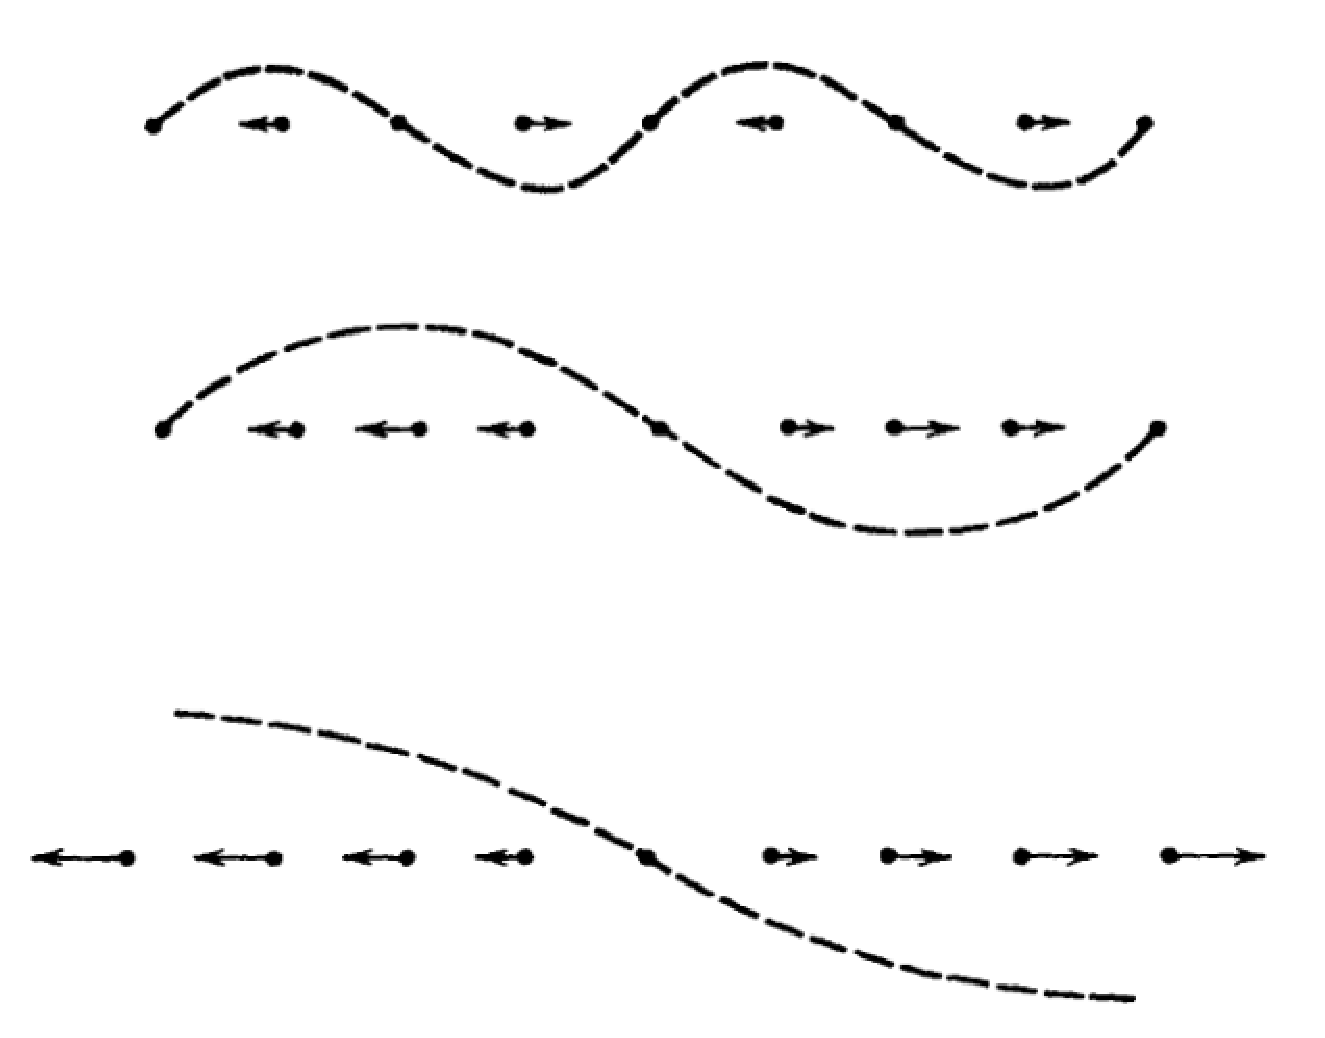
\includegraphics[scale=0.4]{fig1_1.eps} 
	\figcaption{9个原子组成的一维原子链系统的三种简正模。三种模的波长自上而下依次是4个、8个与16个原子间距。虚线表示原子纵向位移的大小。}\label{Fig1.1}
}

各个原子之间相互耦合,全体原子具有的规则的运动模式称为{\it 简正模式}(normal modes),简称简正模\mpar{简正模的概念参见任意一本理论力学教材,例如Herbert Goldstein, Classical Mechanics, 3rd edition,Addison Wesley, \S 6.3, Page 252.}。图\ref{Fig1.1}中显示了三种简正模的运动形式。图中的箭头方向表示原子位移方向,箭头长度表示位移大小。原子来回振动,每过半个周期图中的箭头反向。\mpar{未来会不会有一天教科书可以播放gif动图?}

给出每个原子的位置即描述了系统的原子状态,但更方便的做法是给出各种简正模的瞬时振幅(二者在数学上等价)。这些振幅称为{\it 简正坐标}(normal coordinates),且简正坐标的数量与原子坐标数目相等。

把9个原子组成的系统硬要说成“宏观系统”的话“宏观”与“原子”层面的观测就会没什么区别。为了说明,我们可以将用分辨率很低的“模糊的”仪器进行的观测当作这个系统的宏观测量。于是宏观测量的粗糙性可以类比为用分辨率低的模糊镜片的视野。这种模糊的观测无法分辨图\ref{Fig1.1}中的前两种模式的细节,这些模式不能分辨且宏观上无关。相对而言,第三种模式对应的是系统整体{\it 均匀的整体膨胀或收缩},与前两种不同,这种整体的均匀胀缩即使是“模糊镜片”也能观测到。这一模式的幅度与系统的长度有关(三维情形则为体积)。{\it 长度(体积)是一个热力学变量,空间均匀性(长波模式)结构使得它不会被宏观平均所抹除}。\mpar{原文: {\it The length (of volume) remains as a thermodynamic variable, undestroyed by the spatial averaging, because of its spatially homogeneous (long wavelength) structure.} }

宏观测量的时间平均效果则印证了这些情况。与上述情形类似,系统的每一种简正模有相应的特征频率,长波模式的频率更低。图\ref{Fig1.1}第三种模式的频率是三者中最低的,如果系统原子数非常多,则长波模式的频率极低甚至趋于零(进一步讨论见第\ref{chap21}章)。故而高频的短波模式在时间平均后被抹除,而{\it 与“体积”有关的长波模式频率甚低,它在时间平均下“保留”下来,就像空间平均的情形那样}。

上述简单例子的结论其实非常普遍,只有极少具有高度对称性的原子坐标组合才能在宏观测量的统计平均中生存下来,它们就是宏观热力学量。一些量是力学的:系统的体积、形状参量(如弹性应变)等等,还有的来自电磁学:系统的电或磁的偶极矩、多极矩什么的。{\it 力学(包括弹性力学)研究一部分“保留”下来的的宏观量,电磁学(包括静电学、静磁学与铁磁学)研究另一部分宏观量。}\mpar{原文: {\it The study of mechanics (including elasticity) is the study of one set of surviving coordinates. The subject of electricity (including electrostatics, magnetostatics, and ferromagnetism) is the study of another set of surviving coordinates.} }

{\it 由于宏观测量的粗糙性,系统的宏观描述与大多数原子坐标不直接相关。热力学只关心大量原子坐标的平均后的宏观量。}\mpar{原文:{\it Thermodynamics, in contrast, is concerned with the macroscopic consequences of the myriads of atomic coordinates that, by virtue of the coarseness of macroscopic observations, do not appear explicitly in a macroscopic description of a system.}} 

在诸多宏观系统有大量“隐藏的”原子模式所带来的结果中,最有力的证据是这些模式能储存能量,然后通过“力学模式”(即与宏观力学量有关)的{\it 机械功 (mechanical work)},和“电磁模式”的{\it 电功 (electrical work)}传递能量。前者的典型代表是$-P dV$($P$为压强,$V$为体积),后者的代表为$-E_e d\mathscr{P}$($E_e$为电场,$\mathscr{P}$为电偶极矩)。这些能量传递的完整内容在力学与电磁学文献讨论。{\it 从宏观可观测模式到“隐藏”模式的能量传递同样可能进行。}\mpar{原文:{\it But it is equally possible to 
transfer energy via the hidden atomic modes of motion as well as via those that happen to be macroscopically observable.} } 相应传递的能量称为{\it 热 (heat)}。当然这只是热的形象化描述,在之后正式的体系中将会给出热的可操作的定量定义。

在进行上文的讨论后,下面建立理论所需的概念定义与惯例约定。


\section{热力学系统的组成}
\label{sec1.3}
热力学非常具有普遍性,它可以描述任意复杂体系的所有力学、电磁学与热力学性质。在一开始我们主要关注热学性质,因此系统的力学与电磁性质经常理想化或简化。这很合理,力学基本只考虑不带电而未极化的系统,而电磁学的系统没有弹性形变或其它复杂力学性质。这些学科的普遍性并未因此而降低,在各种性质分别研究透彻后,将它们结合起来处理复杂系统是比较容易的。热力学也一样,一开始我们只考虑力学、电磁学性质最平凡的系统,从而可以专注于热力学的本质内容,再之后容易结合各种理论处理复杂系统。强调一遍:接下来几章所考虑的简单系统{\it 不影响}热力学的普遍性,只是为了研究方便。

(暂时)只考虑如下的{\it 简单系统:宏观均匀、各向同性且不带电,体积足够大可忽略边界效应,而且无外场(如电场磁场重力场)作用。}\mpar{原文:We (temporarily) restrict our attention to {\it simple systems}, defined as {\it systems that are macroscopically homogeneous, isotropic, and uncharged, that are large enough so that surface effects can be neglected, and that are not acted on by electric, magnetic, or gravitational fields.} }

这样一个简单系统没有宏观电磁学量:系统不带电、没有电磁二极四极与多极矩。也没有所有的弹性应变以及其他类似的复杂力学量。体积$V$是一个用得到的力学参量。此外,简单系统还需要一组参量描述其{\it 化学成分}。当系统由多种物质组成时,可以用各组分的原子数作为描述化学成分的参量。为了让原子数参量的数值不那么大,我们采用参量{\it 摩尔数 (mole numbers)},定义为组分的原子数除以Avogadro常数$N_A = 6.02217 \times 10^{23}$.

摩尔数由原子数定义,这超出了纯粹的宏观物理学范围,避免这一情况的等效定义是钦点1摩尔C12同位素的质量为$12 \,\mathrm{g}$. 其它核素的摩尔质量按照C12的比例定义。表1.1列出了部分元素的摩尔质量。

\begin{center}
	\begin{table}[!htbp]
		\centering
		\caption{一些自然环境中元素(同位素混合)的摩尔质量(单位为$\mathrm{g}$). {\it 数据来自the International Union of Pure and Applied Chemistry 1969年数据.}}
		\begin{tabular}{llll}
			\toprule
			\ce{H} & 1.0080 & \ce{F} & 18.9984 \\
			\ce{Li} & 6.941 & \ce{Na} & 22.9898 \\
			\ce{C} & 12.011 & \ce{Al} & 26.9815 \\
			\ce{N} & 14.0067 & \ce{S} & 32.06 \\
			\ce{O} & 15.9994 & \ce{Cl} & 35.453 \\
			\bottomrule
		\end{tabular}
		\label{tab:tt1}
	\end{table}
\end{center}

若系统由$r$种化学成分混合而成,则这$r$种组分各自的{\it 摩尔分数 (mole fractions)}定义为$N_k / (\sum_{j = 1}^r N_j), \quad (k = 1, 2, \dots, r)$, 其中$N_i$为第$i$种组分的摩尔数。所有组分的摩尔分数之和为$1$. 系统的{\it 摩尔体积 (molar volume)}定义为$V / (\sum_{j = 1}^r N_j)$.

宏观参量$V, N_1, N_2, \dots, N_r$有一个超级重要的性质,设想把两个完全相同的系统合体为一个大系统,则大系统的体积是单个子系统体积的两倍,每种组分的摩尔数也是如此。若系统的某个物理量等于每个子系统的该物理量之和,则这个物理量称为{\it 广延量 (extensive parameters)}。广延量在热力学理论中起到关键的作用。

\section{内能}
\label{sec1.4}
能量守恒是物理学最重要的结论之一,这一信念并非一日建成的,而是经历了两个半世纪缓慢而曲折的发展。它的首次提出是在1693年,Leibniz指出地球附近重力场中质点的动能$\frac{1}{2} m v^2$与重力势能$mgh$之和才是守恒的。每当新的相互作用被引入,能量似乎就不守恒了,但是总可以添加新的数学项——一种“新能量”使得能量依然守恒。例如系统带电时,必须引入{Coulomb 相互作用能量}(静电势能)$Q_1 Q_2 / r$以及电磁场能量。1905年,Einstein将能量守恒扩展到相对论领域,引入了相对论性静质能。20世纪30年代Enrico Fermi假设存在中微子,目的是保证核反应过程的能量守恒。现代物理中,能量守恒是物理学基本假设——时间平移对称性的体现,即物理学定律在过去未来从不改变,不在时间平移$(t \to t + \text{常数})$下变化。第21章进一步讨论能量守恒的这一基础。现在我们把能量守恒作为最基本、最普遍、最重要的物理定律就可以了。

宏观系统可以视为大量电子与原子核通过复杂但确定的相互作用(服从能量守恒)结合的整体,由此可推论{\it 宏观系统具有确定的能量值,服从确定的守恒定律}\mpar{原文:{\it macroscopic systems have definite and precise energies, subject to a definite conservation principle.} }。也就是说,我们现在接受明确定义的热力学系统能量作为一种守恒定律的宏观表现形式而存在,它是一种经过高度发展之后的、经测试在原子尺度具有极度精确且明显完整普遍性的能量。\mpar{原文:That is, we now accept the existence of a 
well-defined energy of a thermodynamic system as a macroscopic manifestation of a conservation law, highly developed, tested to an extreme precision, and apparently of complete generality at the atomic level. 
这句话来自百度人工翻译\sout{校对君做了润色},向ta致谢。\sout{我能想象到接到订单的那位翻译蛋疼的神情}}

下面论证热力学能量函数的存在性,但论证方式与历史进程十分不同。因为热力学在原子学说被公认之前就已经蓬勃发展,宏观的能量守恒可以由纯粹的宏观方式验证。这方面的重大突破是1798年Count Rumford观察到大炮钻孔过程中的热效应。Sir Humphry Davy, Sadi Carnot, Robert Mayer, 以及最终的(1840-1850年间)James Joule 在Rumford的基础上形成了完整的论证体系。历史上热的概念的形成过程是科学理论曲折发展的经典案例,体现出新学说被公认所经受的巨大阻力,以及人类在处理精细抽象的问题时的智慧。对此感兴趣的读者可参考D. Roller的著作{\it The Early Development of the Concepts of Temperature and Heat}(Harvard University Press, 1950),或者阅读物理学史文献。

本书不利用Rumford与Joule的实验论证能量函数的{\it 存在性},但第\ref{sec1.7}节会通过这些实验讨论热力学能量的{\it 可测量性 (measurability)}。

无论原子还是宏观层面,具有物理意义的只是能量的差值,而非绝对的值。因此通常选定某一特定状态作为基准态,其能量规定为零。其他状态相对于基准态的能量称为系统的热力学{\it 内能 (internal energy)},通常记作$U$. {\it 内能与体积、摩尔数一样是广延量}。

\section{热力学平衡态}
\label{sec1.5}

宏观系统往往对演化历史有某种“记忆”作用。一杯搅拌过的茶还会旋转一会儿,冷加工过的钢材硬度增加。但记忆终将褪色,扰动总会衰减,内应变屈服成塑性流\mpar{原文:internal strains yield to plastic flow.},不均匀的浓度扩散成一致。系统倾向于演化到与特定的过往条件无关的简单状态。

某些情形中系统很快平息到简单态,另外一些情况的演化过程则慢得要命。但是{\it 所有系统都有向如下特征状态演化的趋势:由系统内部因素决定,与先前的外部影响无关。根据定义,这种简单的终态不依赖时间。这种状态称为平衡态。}\mpar{原文:{\it in all systems there is a tendency to evolve toward states in which the properties are determined by intrinsic 
factors and not by previously applied external influences. Such simple terminal states are, by definition, time independent. They are called equilibrium states.} }

热力学致力于描述系统最终演化到的这种简单、静止的“平衡”状态。

为了将上面的定性陈述转化为定量的正式假设,我们将“简单”的标准设定为使用很少的热力学量即可描述系统。由此引出下面的假设,该假设还受到实验观测的启示,它所导出的理论的正确性验证了它自身的正确性。

\paragraph{假设 \uppercase\expandafter{\romannumeral1}.}
{\it 任意简单系统存在宏观上由内能$U$,体积$V$与各组分摩尔数$N_1, N_2, \dots, N_r$完全确定的宏观状态,称为平衡态。}

\paragraph{Postulate \uppercase\expandafter{\romannumeral1}.}
There exist particular states (called equilibrium states) of simple systems that, macroscopically, are characterized completely by the internal energy $U$, the volume $V$, and the mole numbers $N_1, N_2, \dots, N_r$ of the chemical components. 

\ 

当考虑更一般的、具有更复杂力学电磁学性质的系统时,确定一个平衡态所需的参量也相应增加,例如系统的电偶极矩或弹性应变。新变量的形式体系与简单系统的体积$V$十分相似。

实验中经常要判断一个系统是否处于平衡态,因而是否可以用热力学进行分析。首先可以观察该系统是否不再活动、处于静态,但“不活动”不是平衡态的充分条件。平衡态由广延量$U, V, N_1, N_2, \dots, N_r$完全确定,故而与演化历史无关,这很难在实际中判断。而且许多系统的演化{\it 显然}与历史有关,这些情形促使我们考虑平衡态的意义。例如,两块相同的钢材经历不同的冷加工、淬火和退火过程最终的性质可以十分不同,因而它们不处于平衡态。类似的,玻璃的性质取决于加工过程(如冷却速率),玻璃也不在平衡态。

(基于平衡态的)热力学理论强行分析非平衡态系统就会在将来的报道上出现偏差,实验者根据理论失效(后验标准)判断系统处于非平衡态。

量子统计理论通常会对热力学失效的情形中系统为何不处于平衡态作出更深刻的解释。偶然出现的理论失效往往蕴藏着系统在微观层面未知的复杂过程。例如正氢(orthohydrogen)与仲氢(parahydrogen)\footnote{正氢分子\ce{H2}两个氢核的角动量平行,仲氢的反平行。处于平衡态氢气系统的正氢/仲氢比例应该是定值,但热力学的预言失败了,这促使正氢、仲氢微观性质的研究。}的发现及其微观机制的研究。

一个给定的宏观平衡态(因而给定了系统的边界条件)对应许多微观态,在原子层面上,处于平衡态的系统仍在对应的众多微观态中不断而迅速地转变。转变的速度往往很快,使得宏观测量过程中系统经历各种可能的微观态,这就是系统处于平衡的情况。然而在某些特殊情况下,各微观态的遍历机制失效,系统只能限制在某一特定的微观态的子集中演化转变。或者系统仍可遍历各态,但转变速度较慢,以至于宏观测量结果并非对所有微观态的平均。这些情况的系统都不是平衡态。容易看出,这些奇异情况更容易出现在固体,而非流体(液/气)系统,因为后者相对而言原子的移动性更强,原子随机碰撞强烈消除了微观态遍历限制。

实际上很少有系统处于绝对的平衡态。例如放射性物质的绝对平衡态要求完全衰变为最稳定的同位素,这需要宇宙年龄量级的时间,这种慢的要命的过程可以近似视为平衡态。完成了自发演化、可以用相对较少的参量描述的系统可认为处于{\it 亚稳态 (metastable equilibrium)}。这种稍弱的平衡状态对热力学的应用而言是足够的。

综上,实践中的平衡态判据是循环的。{\it 若热力学理论成功描述了一个系统,则该系统就处于平衡态!}\mpar{原文:{\it Operationally, a system is in an equilibrium state if its properties are consistently described by thermodynamic theory!}}

应该指出,上述\sout{耍流氓的}循环逻辑与力学的情形{\it 没有}不同。例如力学预言质点在已知的引力场中沿特定轨迹运动,如果报道出了偏差,没人会因此否定力学,而是会推测质点受到其他的力。例如如果粒子带电,则考虑电磁力之后动力学预言才正确,这只有通过循环一圈(预言-出了偏差-加上电磁力-预言成功)才推论得知,因而不是先验的。力学系统模型(如质量、转动惯量、电荷、电偶极矩等等)与实验符合之后才是“正确”的。

\section{壁与限制}
\label{sec1.6}
一个热力学系统需要一个“壁”(walls)来将它从周围环境中隔离出来,并为它提供边界条件。通过对壁进行操作,可以改变系统的广延量,以及开始某些演化过程。

通过对壁进行操作而开始的过程通常是某些物理量在不同系统或大系统的子体系之间的重新分布。由此可将热力学壁分为允许或禁止重新分布两种。例如,考虑一个刚性圆筒内部的活塞,如果活塞是固定的,则它是禁止两个子系统的体系重新分布的壁,若活塞可以活动,则允许体积重新分布。刚性圆筒与固定的活塞称为{\it 限制}体积的壁,而可动活塞对体积是非限制的。一般的,将一个系统的某个广延量限制为特定值的壁称为对该广延量有限制,而允许该量自由改变的壁对该广延量是非限制的。

系统的某种化学组分不能渗透的壁限制了该组分的摩尔数;而可以透过的膜对摩尔数无限制。半透膜限制特定组分的摩尔数而对其他成分无影响;一个有孔的壁对任意组分的摩尔数都无限制。

要考虑限制能量的壁是否存在需要先解决能量的可测量性问题,我们下一节就讨论它。

\section{能量的可测量性}
\label{sec1.7}
基于原子层面的能量守恒可以推论出存在守恒的宏观能量函数。为了证明能量具有实际意义,必须说明它是{\it 可控制的(controllable)}与{\it 可测量的(measurable)}。下面首先指出存在测量能量的定量方法,并据此导出热的定量的操作性定义。

论证能量可测量性的关键是绝热壁的存在。下述的简单实验表明存在这种绝热壁。

考虑盛有冰水混合物的容器。实验发现剧烈搅拌容器可使得冰迅速融化,搅拌过程向系统传递了机械功,由此可推论冰的融化与系统能量增加有关。将容器放在夏日的阳光下可以发现冰自然地迅速融化了,该过程外界并未对系统做功,因此可以认为能量通过传热的形式进入系统中。将容器壁从薄金属换成厚玻璃,再换成Dewar瓶壁(两层镀银的玻璃,中间抽真空)会发现冰融化的越来越慢,这强烈暗示金属、玻璃与Dewar壁的隔热性越来越好。机智的实验家可以制造性能超好的隔热壁使得冰的融化速度十分慢,这种壁是理想绝热壁在三次元现实的良好近似。

通常称不透热的壁为{\it 绝热的 (adiabatic)},而允许热传递的壁称为{\it 导热的 (diathermal)}。如果系统的壁既不传递做功也不导热,则它可以{\it 限制系统的能量}。若系统的壁限制能量、体积与所有组分的摩尔数,则称这个系统是{\it 封闭的 (closed)}\footnote{本书的封闭性的定义与化学中的惯例不同,化学的封闭性只是限制系统组分的摩尔数不变。}。

利用上述几种壁可以论证宏观热力学能量的{\it 可控制性},比如可以用绝热壁关住能量,用透热壁使能量流动。再比如将系统用限制能量的壁封印起来的话,该系统明天的能量也可以确定。没有这些壁的话,热力学就成了空谈的纯理论了。

下面讨论能量的{\it 可测量性},更确切的说,是讨论(具有物理意义的)能量差的可测量性。被绝热壁包围的简单系统只可能通过做功的方式向它传递能量。机械功可根据力学理论计算。例如压缩活塞做的功等于力乘以位移,用杆搅拌的功等于力矩乘以角位移。这种情况的功在力学里已经完备地讨论了定义与测量方法。由此可得,{\it 如果系统被绝热壁包围,并通过做机械功从一个状态达到另一个状态,}则这两个状态的能量差即为所做机械功的值。\mpar{原文:we are able to measure the energy difference of two states {\it provided that one state can be reached from the other by some mechanical process while the system is enclosed by an adiabatic impermeable wall.}} 

例:考虑刚性绝热容器中达到平衡态的冰水混合物系统。在壁上开一个小洞穿过一个杆,杆的一侧是桨,另一侧是曲柄,这样就能通过转动曲柄对系统做机械功,机械功等于力矩乘以角位移。转一段时间后,系统达到新的平衡态(一些冰融化了)。系统末态减初态的能量差即为转动曲柄做的功。

还有一个问题。将系统由绝热壁包围\mpar{如无特别说明,本节涉及的壁都是不可透过物质的(impermeable)。},初状态任意,它能否只通过做机械功达到任意指定的末态?这要借助Joule完成的实验,他的工作表明{\it 绝热系统摩尔数$N_1, \dots, N_r$相等的任意两个状态,都存在力学过程将它们联系起来}。\mpar{原文:{\it system enclosed by an adiabatic impermeable wall any two equilibrium states with 
the same set of mole numbers $N_1, N_2,..., N_r$. can be joined by some possible mechanical process.} } Joule还发现给定(绝热系统的)两个状态(记作$A, B$)后,从$A \to B${\bf 或者}$B \to A$的力学过程至少存在一个,但其中的某一个(比如$A \to B$)可能不存在。我们的目的是测量状态的能量差,因此存在一个过程就够用了。综上,{\it 借助机械功可以测量摩尔数相同的任意两个状态的能量差。}

Joule观察到的只有$A \to B$或$B \to A$一个过程存在的情形具有深刻意义。这两个状态的不对称是{\it 不可逆性 (irreversibility)}概念的体现,后面会深入讨论。

上述测量能量差的方法的唯一限制是初末状态摩尔数相同。这可以由如下方式解决:考虑由挡板(物质不可透过)隔开的两个子系统,它们的相对于基准态的能量可由上述方法测出。移除挡板,子系统混合,并且二者的总能量守恒。因此混合系统的终态能量等于两个子系统的初态能量之和。这样就可以测量摩尔数不同的状态间的能量差。

总结:{\it 利用绝热壁与机械功可以测量热力学系统任意状态相对于基准态的能量。}\mpar{原文:{\it by employing adiabatic walls and by measuring only mechanical work, the energy of any thermodynamic system. relative to an appropriate reference state, can be measured. } }

\section{热的定量定义}
\label{sec1.8}
利用任意两个平衡态的能量差的可测量性,可以对热进行定量定义:{\it 系统在某一(摩尔数不变)过程中外界流入系统的热量定义为系统末态与初态的能量差减去外界对系统做的功。}\mpar{原文:{\it The heat flux to a system in any process (at constant mole numbers) is simply the difference in internal energy between the final and initial states, diminished by the work done in that process. } }

设系统经某一过程由初态$A$演化为末态$B$,该过程中外界对系统做的功以及外界传递给系统的热量是多少?前者根据力学理论不难计算。根据\ref{sec1.7}节介绍的方法可得能量差$U_B - U_A$,从能量差中减去机械功即可得该过程中传递给系统的热流。

应该指出,相同的初末状态对应的不同过程的做功大小可以不同,同样,传热大小也可以不同,但是做功与传热的和——能量差$U_B - U_A$在初末态给定后对所有过程都是相等的。计算能量差只需给定初末状态,而计算做功、传热大小必须给出联系初末态的特定过程。

外界对简单热力学系统通过改变体积所做的准静态功为:
\begin{equation}
\label{equ1.1}
	\dbar W_M = -P dV
\end{equation}
其中$P$为系统压强。上式不难从力学导出,必须强调上式只适用于{\it 准静态过程 (quasi-static processes)}。准静态过程的准确定义在\ref{sec4.2}节讨论,这里只进行定性解释。考虑一个带有可移动活塞的气缸,气缸内封闭有一定气体。迅速压动活塞,则在活塞附近的气体立即获得动能,气体出现湍流,压强无法定义。这种过程不是准静态的,对系统做的功也不能由\eqref{equ1.1}式计算。如果以极其慢(准静态地)速率推动活塞,则系统在每一时刻都可视为处于静平衡态,\eqref{equ1.1}式可以使用。粗略地说,“无穷慢”即为准静态过程的本质。

\eqref{equ1.1}式的符号惯例值得注意。若系统的能量增加,则外界对系统做正功。若系统体积减少,则外界对系统做正功,使系统的能量增加,因此\eqref{equ1.1}式等号右侧有个负号。

利用准静态功的定量表述$\dbar W_M = -PdV$可导出传热的定量公式,一个摩尔数不变的无穷小准静态过程中传递给系统的{\it 准静态热量 (quasi-static heat)}$\dbar Q$定义为:
\begin{equation}
\label{equ1.2}
	\dbar Q = dU - \dbar W_M, \quad \text{摩尔数不变。}
\end{equation}
或者:
\begin{equation}
\label{equ1.3}
	\dbar Q = dU + P dV, \quad \text{摩尔数不变。}
\end{equation}
{\it 热量 (heat)}与{\it 热流 (heat flux)}这两个术语经常混用,因为热量就像功那样,是能量的{\it 传递 (transfer)}形式。能量传入系统之后就不能分辨是通过做功还是传热传给系统的,尽管$dU$分为$\dbar Q$与$\dbar W_M$两部分,但能量$U${\it 不能}分为“做功”部分与“传热”部分。我们采用符号$\dbar$表示无穷小做功与传热,$\dbar Q$与$\dbar W_M$称为{\it 不完整微分 (imperfect differentials)}。$\dbar W_M$与$\dbar Q$沿某一特定过程进行积分得到{\it 该过程}的做功与传热值,而它们的和——能量差$\Delta U$与具体过程无关(只与初末状态有关)。

热量,功与能量的概念可通过如下的类比来说明。设一位农场主有个池塘,一条溪流注入池塘,另一条从池塘流出。池塘还通过降雨获得水分、通过蒸发流失水分(“负降雨”)。将池塘比作热力学系统,水量视为系统内能,溪流注入流出类比做功,降雨蒸发当做传热。

首先,在任何时刻,池塘的水不能分成来自降水与来自溪流的部分。{\it 降雨}只是水{\it 转移}的形式。

然后考虑测量池塘水量的方法。可以使用流量计测量流入流出池塘的溪流水量,但是对降雨而言没有那样的雨量计。为了测量降雨量,可以用防水布将池塘覆盖,使得降雨和蒸发不能改变水量。将一带刻度的长直杆垂直插入池塘以记录水位变化,通过在两条溪流筑坝即可控制池塘水位,结合流量计与刻度杆即可测定池塘水量。因此在防水布的帮助下,池塘任意水位的水量都可测定\mpar{当然,就像\ref{sec1.7}节只是测定系统任意状态{\bf 相对于基准状态}的能量那样,这里只测定池塘的任意水位相对于某一基准水位对应的水量。}。

把防水布撤去从而使降水可以影响池塘水量,要得到某一过程中降水导致的水量变化,可以通过如下间接方式。首先在刻度杆上读出水位的变化,从而水量的变化可以由上一段的方法得出。然后根据流量计测量溪流造成水量的变化。水量的变化减溪流造成的变化即为降水量。读者不难看出其中的类比关系。

因为做功与传热都是能量传递的形式,故功和热量的都是能量的单位。能量在cgs单位制\mpar{cgs: centimeter-gram-second单位制,或者厘米-克-秒单位制,又称高斯单位制。}中的单位是erg(尔格),在mks单位制\mpar{mks: metre-kilogram-second单位制,或者米-千克-秒单位制,又称国际单位制。}中为joule (焦耳),记作J,二者的关系为$1\, \mathrm{J} = 10^7\, \mathrm{erg}.$

常用的能量单位还有calorie(卡,1 cal = 4.1858 J)\footnote{营养学家习惯把一千calorie简记为``Calorie''(这使得能量的数值合适不至于太大),但要命的是他们经常忘了大写字母C,于是一千calorie成了一``calorie''!}。历史上,calorie是在热与功的关系澄清之前所用的热量单位,直到现在,还有人只用calorie计量热量、用joule计量功。然而calorie与joule都是能量单位,它们描述功与热量都是可以的。

其他的能量单位制还有英国热量单位(the British thermal unit, Btu),升-大气压单位(liter-atmosphere),英尺-磅单位(foot-pound)与瓦特-时单位(watt-hour)。各单位制能量单位间的转换参见本书封底。

{\bf {\large 例 1}}
\ 

带有可移动活塞的气缸内封印着一定气体。通过观测发现,气体在绝热过程中满足:
\[
	P^3 V^5 = \text{constant}, \quad (\dbar Q = 0)
\]

\begin{enumerate}
	\item[(a)] 求下图$ADB, ACB, A \stackrel{ \text{直线} }{\longrightarrow} B$三个过程中外界对系统做的准静态功、外界传递给系统的热量。


	{
		\centering
		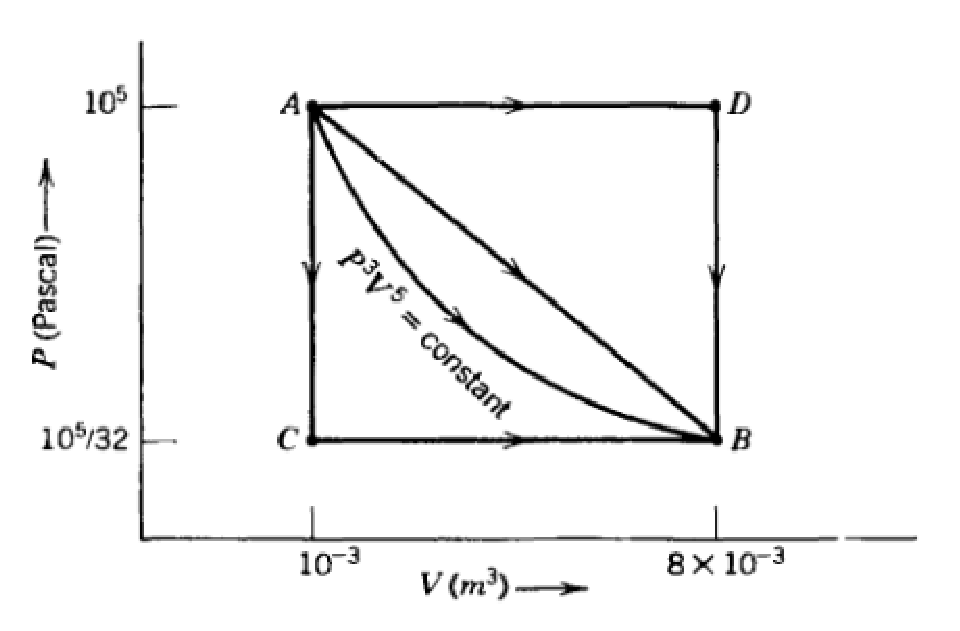
\includegraphics[scale=0.7]{fig1_8.eps}
		\notag
	}

	在$ADB$过程中气体保持压强不变($P = 10^5 \, \mathrm{Pa}$)被加热,从初始体积$10^{-3} \, \mathrm{m}^3$变为末态体积$8 \times 10^{-3} \, \mathrm{m}^3$. 然后保持体积不变,将气体冷却至压强降为$10^5 / 32 \, \mathrm{Pa}$。同样,其他过程($ACB, AB$)的具体内容由图不难看出。

	\item[(b)] 在系统内安装一个由发动机驱动的桨,在发动机提供的力矩作用下桨以均匀角速度$\omega$转动,观测到气体系统(体积不变)压强的变化率为:
	\[
		\frac{dP}{dt} = \frac{2}{3} \frac{\omega}{V} \times \text{力矩}
	\]
	求证系统任意两个体积相等的状态的内能差可通过该过程计算。算出$U_C - U_A$和$U_D - U_B$.

	这个过程只能单向进行(只能从$P-V$图垂直向上而不能向下进行),这是为啥?

	\item[(c)] 求证系统的任意两个平衡态(即$P-V$图中的任意两点)可通过(a)、(b)描述的两个过程联系起来。计算$U_D - U_A$.

	\item[(d)] 计算图中$A \to D$过程外界对系统做的功$W_{AD}$以及传递给系统的热$Q_{AD}$. 计算$D \to B, C \to A$过程同样的量,并说明这些计算结果与(a)一致。
\end{enumerate}

读者在参考下面的答案{\it 之前}应该先尝试解答这些题目。

\ 

{\it \large 解答}

\begin{enumerate}
	\item[(a)] 
		利用绝热条件$Q = 0, \Delta U = W$以及$P^3 V^5 = \mathrm{constant}\, \quad (Q = 0)$可得:
	\begin{align*}
		U_B - U_A &= W_{AB} = -\int_{V_A}^{V_B} PdV = -P_A \int_{V_A}^{V_B} \left( \frac{V_A}{V} \right)^{5/3} dV \\
		&= \frac{3}{2} P_A V_A^{5/3} \big( V_B^{2/3} - V_A^{2/3} \big) \\
		&= \frac{3}{2} (25 - 100) \,\mathrm{J} = -112.5\, \mathrm{J}.
	\end{align*}
		考虑$ADB$过程:
		\begin{align*}
			W_{ADB} &= -\int PdV = -10^5 \times (8 \times 10^{-3} - 10^{-3}) \,\mathrm{J} = -700 \,\mathrm{J} \\
			U_B - U_A &= W_{ADB} + Q_{ADB} \\
			Q_{ADB} &= (-112.5 + 700) \,\mathrm{J} = 587.5 \,\mathrm{J}.
		\end{align*}
		尽管能算出$Q_{ADB}$,但不能分别得到$Q_{AD}, Q_{DB}$,因为还不知道$U_D - U_A$.

		其他过程的计算同理。答案是$W_{ACB} = -21.9 \,\mathrm{J}, Q_{ACB} = -90.6 \,\mathrm{J}; W_{AB} = -360.9 \,\mathrm{J}, Q_{AB} = 248.4 \,\mathrm{J}$.
	\item[(b)] 
		电动机的力矩使桨旋转角度$d\theta$传递给系统的能量\footnote{注意电动机传递能量给系统既不是做功也不是传热的方式——这是一种{\it 非准静态 (non-quasi-static)}的能量传递。 }为$dU = \text{力矩} \times d\theta$, 另外$d\theta = \omega dt$,因此
		\begin{align*}
			dP &= \frac{2}{3} \frac{1}{V} \cdot \text{力矩} \cdot \omega dt \\
			&= \frac{2}{3} \frac{1}{V} dU \\
		\end{align*}
		整理得
		\[
			dU = \frac{3}{2} VdP
		\]
		$dU = \text{力矩} \times d\theta \to dU \geq 0$($d\theta$与力矩符号相同),再结合$V > 0$可得$dP \geq 0$,因此该过程只能向压强增大的方向单向进行。

		\begin{align*}
			U_A - U_C &= \frac{3}{2} V (P_A - P_C) = \frac{3}{2} \times 10^{-3} \times \left( 10^5 - \frac{1}{32} \times 10^5 \right) = 143.5 \,\mathrm{J} \\
			U_D - U_B &= \frac{3}{2}
		\end{align*}
	\item[(c)]
		任意给定$P-V$图上两点,为了将它们联系起来,过其中任意一点画一条绝热线(绝热过程对应的线),再过另一点画等容线($V = \text{常数}$),这两条线相交,于是两个过程联系起来。

		前面已经利用绝热过程求出$U_B - U_A = -112.5 \,\mathrm{J}$,利用不可逆的搅拌过程求出$U_D - U_B = 1162.5 \,\mathrm{J}$。因此$U_D - U_A = 1050 \,\mathrm{J}$。等价地,可以将状态$A$设为基准态,则
		\[
			U_A = 0, \quad U_B = -112.5 \,\mathrm{J}, \quad U_C = -145.3 \,\mathrm{J}, \quad U_D = 1050 \,\mathrm{J}.
		\]
	任意状态的内能$U$都可以求出。
	\item[(d)]
		已经计算出了$U_D - U_A$以及$W_{AD}$,由此可得$Q_{AD}$:
		\begin{align*}
			U_D - U_A &= W_{AD} + Q_{AD} \\
			1050 \,\mathrm{J} &= -700 \,\mathrm{J} + Q_{AD} \\
			Q_{AD} &= 1750 \,\mathrm{J}
		\end{align*}
		同样
		\begin{align*}
			U_B - U_D &= W_{DB} + Q_{DB} \\
			-1162.5 \,\mathrm{J} &= 0 + Q_{DB}.
		\end{align*}
		为了检验,计算$Q_{AD} + Q_{DB} = 587.5 \,\mathrm{J}$,等于在(a)中计算的$Q_{ADB}$,nice!
\end{enumerate}

\subsection*{习题}\mpar{译者水平有限只敢列出原文有答案的习题的解题过程……(没答案的不知道对错不敢放上去)}
\begin{enumerate}
	\item[1.8-1.]
		计算本节例1中系统状态$(P = 5 \times 10^4 \,\mathrm{Pa}, V = 8 \times 10^{-3}\, \mathrm{m}^3)$对应的内能。

		{\it
			以状态$A$为参考状态,即设$U_A = 0$.

			记$(P = 5 \times 10^4 \,\mathrm{Pa}, V = 8 \times 10^{-3}\, \mathrm{m}^3)$为状态$E$. 因$V_B = V_E$,故可通过例1(b)描述的不可逆搅拌过程从$E$演化到$B$态:
			\begin{align*}
				E \stackrel{{\text{不可逆搅拌}} }{\longrightarrow} B \\
				U_B - U_E &= \frac{3}{2} V_E (P_B - P_E) \\
				&= \frac{3}{2} \times 8 \times 10^{-3} \times \left( \frac{1}{32} \times 10^{5} - 5 \times 10^{4} \right) \,\mathrm{J} \\
				&= -562.5 \,\mathrm{J}.
			\end{align*}
			由例1(c),以$A$为参考态时,$U_B = -112.5 \,\mathrm{J}$,故 
			\begin{equation*}
				U_E = \big(-112.5 - (-562.5) \big) \,\mathrm{J} = 450 \,\mathrm{J}.
			\end{equation*}
		}
	
	\item[1.8-2.]
		还是例1的条件。记上一问的状态$(P = 5\times 10^4 \,\mathrm{Pa}, V = 8 \times 10^{-3} \,\mathrm{m}^3)$为$X$,计算系统从状态$A$沿$P-V$图的直线演化到状态$X$过程中吸收的热量。

	\item[1.8-3.]
		某一气体系统的能量为:
		\[ U = 2.8 PV + \text{constant}. \]
		系统的初始状态为$P = 0.2\, \mathrm{MPa}\ (10^{6} \mathrm{Pa}), V = 0.01\, m^3$,对应下图中的A点。系统经历图中的循环过程($A \to B, B \to C, C \to A$)。计算每个过程中系统的吸热量$Q$与外界对系统做的功$W$。
		
		
		{
			\centering
			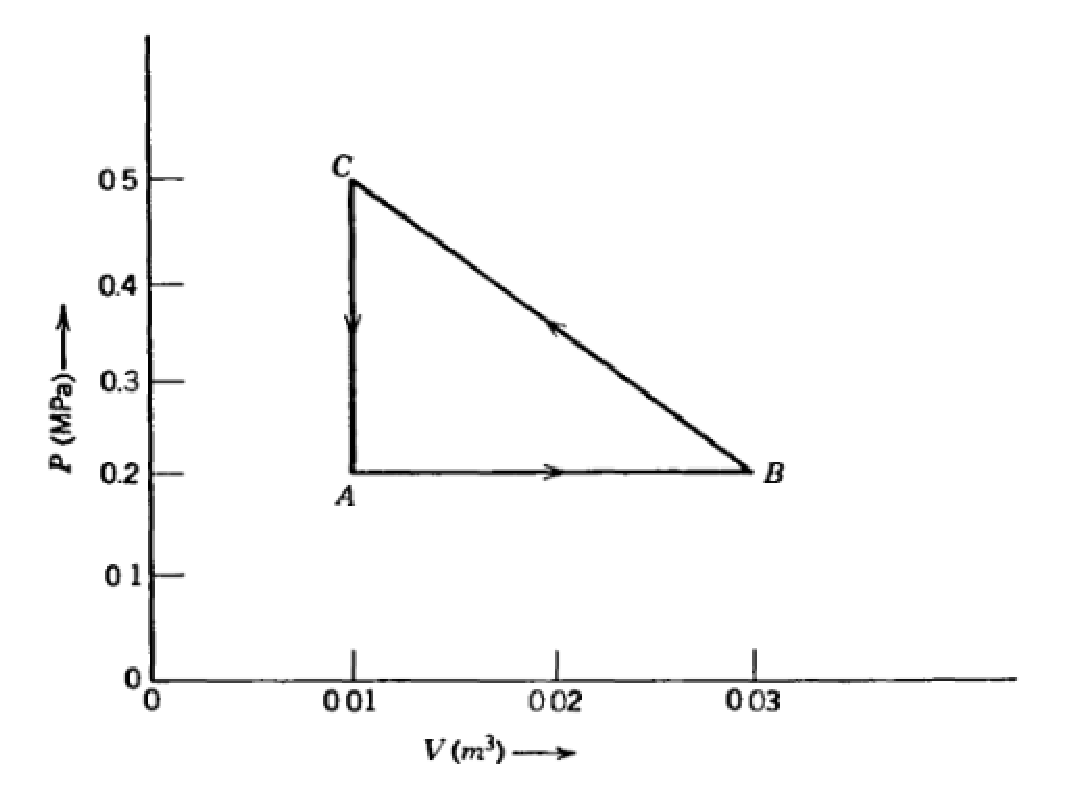
\includegraphics[scale=0.6]{fig1_8_3.eps}
			\notag
		}
		
		
		{\it
			以$B \to C$过程为例(答案只给了$BC$过程的……)
		
			状态$B$:$V = 0.03\, \mathrm{m}^3, P = 0.2 \mathrm{MPa}$.

			状态$C$:$V = 0.01 \,\mathrm{m}^3, P = 0.5 \,\mathrm{MPa}.$

			直线 $BC$: $P = (-15\, \mathrm{MPa \, m^{-3}}) V + 0.65\, \mathrm{MPa}$.

			\[ W_{BC} = -\int_{V_B}^{V_C} PdV = -\int_{0.03}^{0.01} (-15V + 0.65) dV = 7 \times 10^3 \,\mathrm{J}. \]

			\[ U_C - U_B = 2.5(P_C V_C - P_B V_B = 2.5(0.5\times 0.01 - 0.2 \times 0.03) \,\mathrm{MJ} = -2.5 \times 10^3 \,\mathrm{J}. \]

			\[ Q_{BC} = (U_C - U_B) - W_{BC} = (-2.5 \times 10^3) \,\mathrm{J} - 7 \times 10^{3} \,\mathrm{J} = -9.5 \times 10^3 \,\mathrm{J}. \]
		}

	\item[1.8-4.]
		求习题1.8-3中的系统在绝热过程中的$P-V$曲线,即求$P = P(V)$使得沿这条线的过程满足$\dbar Q = 0$。

		{\it
			外界对系统做的功为
				\[ W = -\int_{V_0}^{V} P(V') \, dV'. \]
			绝热过程中系统吸热$Q = 0$,故内能变化量$U = W$。由1.8-3中条件\mpar{$U = 2.5 PV + \mathrm{constant}$. }可知,初末状态的内能差为:
				\[ U = 2.5(P V - P_0 V_0). \]
			联立得
				\begin{align*}
					2.5 (PV - P_0 V_0) = -\int_{V_0}^V P(V') \, dV' \\
					= 2.5 \left(P + \frac{dP}{dV} V \right) = -P(V) \\
					\frac{dP}{dV} = -\frac{7}{5} \frac{P(V)}{V} \\
					\to P \propto V^{-7/5} \\
					\to P^5 V^7 = \mathrm{constant}.
				\end{align*}
		}
	\item[1.8-5]
		单位摩尔数物质的某系统的内能为
		\[ U = AP^2 V. \]
		其中$A$是正的常数,量纲为$[\mathrm{P}]^{-1}$. 求$P-V$图绝热线的形式。

	\item[1.8-6]
		实验观测发现某系统保持体积$V_0$不变,压强从$P_0$变化到任意值$P'$时,系统吸收的热量为
		\[ Q' = A(P' - P_0) \quad(A > 0). \]
		此外,系统在绝热过程满足:
		\[ P V^\gamma = \text{constant} \quad (\gamma\text{是正的常数}) \]
		求任意状态的内能$U(P, V)$. (用已知量$P_0, V_0, A, U_0 \equiv U(P_0, V_0)\text{与} \gamma$,当然还有自变量$P, V$表示)

		{\it
			\[ A: (V_0, P_0), \quad B: (V_0, P_B), \quad C: (V, P). \]
			构造如下状态使得系统从初态$A$演化到末态(任意状态)$C$:
			\[ A \stackrel{\text{定容过程}}{\longrightarrow} B \stackrel{\text{绝热过程}}{\longrightarrow} C. \]

			$A \stackrel{\text{定容过程}}{\longrightarrow} B$: 
				
			$W_{AB} = 0, Q_{AB} = A(P_B - P_0)$,
			\[ U_B - U_A = W_{AB} + Q_{AB} = A(P_B - P_0). \]

			$B \stackrel{\text{绝热过程}}{\longrightarrow} C$: 
				
			$Q_{BC} = 0$.
			\[ P V^\gamma = P_B V_0^\gamma \to P = \frac{P_B V_0^\gamma}{V^\gamma}. \]
			\[ W_{BC} = -\int_{V_0}^{V} \frac{P_B V_0^\gamma}{V'^\gamma} \,dV' = -P_B V_0^\gamma \frac{V^{-\gamma + 1} - V_B^{-\gamma + 1}}{-\gamma + 1}. \]
			\[ U - U_B = Q_{BC} + W_{BC} = -P_B V_0^\gamma \frac{V^{-\gamma + 1} - V_0^{-\gamma + 1}}{-\gamma + 1}. \]

			因此初末状态内能差为
			\begin{align*}
				U - U_0 &= (U - U_B) + (U_B - U_A) \\
				&= -P_B V_0^\gamma \frac{ V^{-\gamma + 1} - V_0^{-\gamma + 1} }{-\gamma + 1} + A(P_B - P_0).
			\end{align*}
			将$P_B = PV^\gamma / V_0^\gamma$带入得
			\begin{align*}
				U - U_0 &= -P V^\gamma \frac{V^{-\gamma + 1} - V_0^{-\gamma + 1} }{-\gamma + 1} + A( \frac{PV^\gamma}{V_0^\gamma} - P_0) \\
				&= A(Pr^\gamma - P_0) + PV \frac{1 - r^{\gamma - 1}}{\gamma - 1}. \quad (r \equiv \frac{V}{V_0})
			\end{align*}
		}

		\item[1.8-7]
			实验观测发现,某具有2摩尔单一组分的系统内能$U$与压强、体积的关系为:
			\[ U = APV^2. \quad (N = 2) \]
			注意,如果把系统的体积、内能与摩尔数均变为原来的两倍,压强不会改变。求任意摩尔数$N$的$U = U(P, V, N)$.
\end{enumerate}


\section{热力学基本问题}
\label{sec1.9}
现在准备工作已经完成,可以开始讨论热力学的基本问题以及它的解了。

回顾准备过程,我们发现仅仅选择了热力学变量就可以得到大量有意义的结果,热力学变量的选择标准揭示了测量的作用,宏观变量与杂乱的微观变量之间的区别体现出功与热的不同,热力学变量能否完整描述系统定义了平衡态。现在,热力学变量可以为热力学基本问题的解决提供框架。

实际上,有一个中心问题定义了热力学理论的核心,所有热力学的结果都可以从该问题的答案演化产生。

{\it 这独一无二、无所不包的热力学核心问题是——在移动一个封闭的复合系统的内部限制之后,确定系统最终演化到的平衡态。}\mpar{原文:{\it The single, all-encompassing problem of thermodynamics is the determination of the equilibrium state that eventually results after the removal of internal constraints in a closed, composite system.}}

考虑封闭气缸内由活塞分隔的两个简单系统。设气缸壁与活塞刚性、绝热、不能透过物质,并且活塞被固定住,则每个系统都是封闭的。如果去掉活塞的固定,一般情况下活塞会移动到新平衡位置。同样,去掉固定住的活塞绝热的限制,两个系统间的能量会重新分布。如果在活塞上打孔,则两系统的物质会重新分布(从而能量也会)。上述几种情形中,限制条件的去除使某些自发演化过程开始,当两个系统进入新平衡态之后,它们由热力学量$U^{(1)}, V^{(1)}, N_1^{(1)}, \cdots$以及$U^{(2)}, V^{(2)}, N_1^{(2)}, \cdots$描述。热力学的基本问题就是计算这些参量的值。

{{
	\centering
	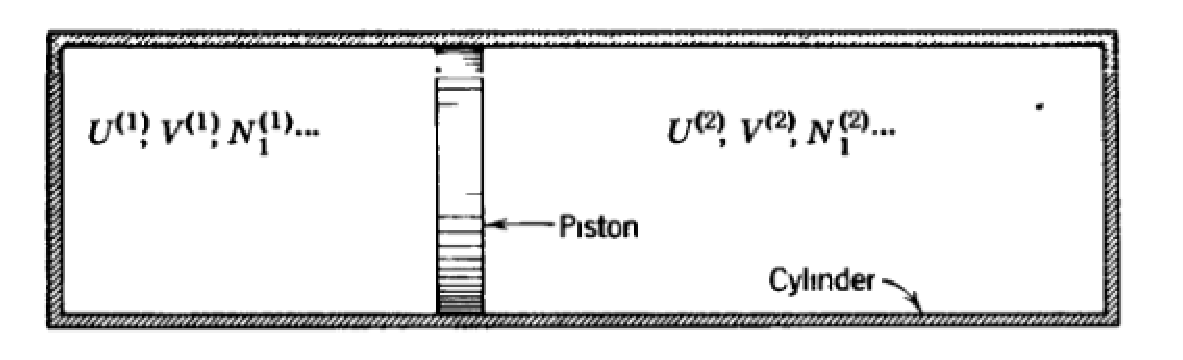
\includegraphics[scale=0.7]{fig1_2.eps}
	\figcaption{}
}}

在下一节讲述解决此问题的定量方法之前,我们用更一般的方式重述基本问题,无需借助气缸与活塞。给定两个或多个简单系统,它们整体可以视为一个{\it 复合 (composite)}系统。封闭的复合系统被限制总能量、总体积与总摩尔数的壁{\it 包围},而封闭复合系统的简单子系统无需是封闭的,比如复合系统内部的活塞可以透热或者有个洞。复合系统的{\it 内部 (internal)}限制阻止了各简单系统之间的能量、体积或物质重新分布。一个封闭的复合系统在某一内部限制下达到平衡态,若将该内部限制去掉,则之前禁止的某些状态现在可能达到。这一过程使系统达到新平衡态。热力学的基本问题就是预言这一新平衡态。

\section{最大熵假设}
\label{sec1.10}
由热力学的中心原理出发可解决热力学基本问题,而从实验观测归纳出中心原理的过程相当微妙。这一人类智慧的杰作在历史上最终由Caratheodory分析完成。以Josiah Willard Gibbs为先驱的统计力学方法需要熟练的归纳性灵感。The symmetry-based foundations to be developed in Chapter 21 will provide retrospective understanding and interpretation, but they are not yet formulated as a deductive basis. 
因此我们仅仅将热力学基本问题的解决方法以一系列后验性的\mpar{意思是假设的正确性由它导出的结论的正确性(后验性地)验证。}假设给出,而非以先验的证据的形式。实际上在考虑到基本问题{\it 最简单的形式解}之后,这些假设是非常自然的。On this basis alone the problem {\it might} have been solved; 将一个问题的最简形式解作为试探性的假设是理论物理学常见而管用的套路。

平衡态最简单而又靠谱的判断标准是什么?物理学的人生经验告诉我们——平衡的黄金准则是让某个量取极值。亦即,我们猜想,处于平衡终态系统的各广延量($U, V, N, \dots$)使得某个函数取最大值\footnote{其实取最小值也可以,假设取最大值只是惯例,两个选项只差一个负号,不影响理论的逻辑结构。}。再(乐观地)假设这个函数有非常好的数学性质\mpar{数学家眼中搞物理的耍流氓系列},这样能保证所导出的理论的简洁性。如前述,下面提出一系列(三个,\ref{sec1.5}节还有一个)假设以解决热力学基本问题。

{\bf 假设 \uppercase\expandafter{\romannumeral2}. } {\it 任意复合系统的平衡态都存在一个广延量的函数(称为熵,记作$S = S(U, V, N_1, \dots, N_r)$),熵在系统处于任意平衡态时定义为有如下性质:

在系统的广延量没有内部限制时,平衡态对应的广延量使得熵函数取最大值。}


{原文:{\it There exists a function (called the entropy S) of the extensive parameters of any composite system, defined for all equilibrium states and 
having the following property: The values assumed by the extensive parameters in the absence of an internal constraint are those that maximize the entropy over the manifold of constrained equilibrium states. }}

必须强调,上面的假设只定义了熵在系统处于平衡态的性质,丝毫未涉及非平衡态。没有内部限制的系统可以处于任何状态,而{\it 其中每个状态都可以当存在某些限制时达到}。这种有限制的平衡态的熵在上面已经被定义,且其中某一平衡态的熵最大。在没有限制的情况下,系统的平衡态就是该最大熵对应的平衡态。

设想两个被透热壁分隔的子系统,总能量$U$在两个子系统之间如何分配?首先考虑将透热壁换为绝热壁的复合系统,子系统的能量分别为$U^{(1)}, U^{(2)}$(当然$U^{(1)} + U^{(2)} = U$)。每个有限制的平衡态$(U^{(1)}, U^{(2)})$对应一个熵,熵在某个特定的$U^{(1)*}, U^{(2)*}$处取最大值。因此当绝热的限制去掉,即子系统由透热壁分隔时,复合系统的平衡态对应的能量分配为$U^{(1)*}, U^{(2)*}$。

热力学的所有问题都可以从\ref{sec1.9}节介绍的基本问题导出。若系统的熵关于广延量的函数关系已知,则基本问题就可迎刃而解。熵关于广延量的函数关系式称为{\it 热力学基本关系 (fundamental relation)}。因此{\it 若系统的基本关系已知,则该系统所有热力学信息都可从中得出}。

上文陈述的内容极其重要。基本关系包含了系统所有的热力学信息——它等价于系统所有的数据、图表等任何描述热力学性质的内容。若系统的基本关系已知,则任何热力学性质都可精确求出。


{\bf 假设 \uppercase\expandafter{\romannumeral3}. } {\it 
复合系统的熵等于所有子系统的熵之和,即熵具有可加性。

熵是连续、可微,且关于内能单调递增的函数。}

由该假设立即可导出一些熵的数学性质。熵具有可加性,即复合系统的熵$S$是各子系统的熵$S^{(\alpha)}$之和:
\begin{equation}
\label{equ1.4}
	S = \sum_\alpha S^{(\alpha)}.
\end{equation}
每个子系统的熵是各自的广延量的函数:
\begin{equation}
\label{equ1.5}
	S^{(\alpha)} = S^{(\alpha)} \Big( U^{(\alpha)}, V^{(\alpha)}, N_1^{(\alpha)}, \dots, N_r^{(\alpha)} \Big).
\end{equation}
将可加性应用于空间上分开的几个子系统,可得熵的如下性质:{\it 简单系统的熵是广延量的一阶齐次函数}。也就是说,将系统的所有广延量变为$\lambda$倍,则熵也变为$\lambda$倍,用公式表示为:
\begin{equation}
\label{equ1.6}
	S(\lambda U, \lambda V, \lambda N_1, \dots, \lambda N_r) = \lambda S(U, V, N_1, \dots, N_r).
\end{equation}

熵关于内能单调递增意味着偏导数大于零:
\begin{equation}
\label{equ1.7}
	\left( \frac{\partial S}{\partial U} \right)_{V, N_1, \dots, N_r} > 0.
\end{equation}
下一章会看到,上式左侧的倒数即为温度$T$的定义,因此根据该假设,温度是非负的\footnote{这个偏导数为负数(即温度为负数)可能性的讨论可见N F Ramsey, {\it Phys. Rev.} 103, 20 (1956). 负温度的真实系统并非处于平衡态,因此与\eqref{equ1.7}式不矛盾。这种状态只能在非常特殊的系统(例如孤立自旋系统)中实现,并且很快就衰变掉了。然而这种负温度状态的研究具有统计力学意义,例如阐明统计力学中温度的概念。 }。

熵的连续、可微性以及关于内能的单调性意味着熵函数可以转化为内能关于$S, V, N_1, \dots, N_r$的{\it 单值、连续以及可微的}函数,即
\begin{equation}
\label{equ1.8}
	S = S(U, V, N_1, \dots, N_r)
\end{equation}
可以唯一地解出具有如下形式的内能函数$U$:
\begin{equation}
\label{equ1.9}
	U = U(S, V, N_1, \dots, N_r).
\end{equation}
\eqref{equ1.8}与\eqref{equ1.9}式是基本关系的两种形式,它们中的每一个都包含了系统的{\it 所有}热力学信息。

熵的广延性表明$N$摩尔物质的系统的熵等于$1$摩尔系统的熵的$N$倍,这用基本关系表示为:
\begin{equation}
\label{equ1.10}
	S(U, V, N_1, \dots, N_r) = N\, S \left( \frac{U}{N}, \frac{V}{N}, \frac{N_1}{N}, \dots, \frac{N_r}{N} \right).
\end{equation}
上式即为\eqref{equ1.6}式中的因子$\lambda$取$1/N \equiv 1 / \sum_k N_k$的结果。对于单一组分的简单系统有:
\begin{equation}
\label{equ1.11}
	S(U, V, N) = N\, S \left( \frac{U}{N}, \frac{V}{N}, 1 \right),
\end{equation}
$U/N$是单位摩尔数的内能,将它记作$u$:
\begin{equation}
\label{equ1.12}
	u \equiv \frac{U}{N},
\end{equation}
同样,单位摩尔数对应的体积$V/N$记作$v$:
\begin{equation}
\label{equ1.13}
	v \equiv \frac{V}{N}.
\end{equation}
因此$S(U/N, V/N, 1) \equiv S(u, v, 1)$是单位摩尔粒子数的系统的熵,记作$s(u, v)$:
\begin{equation}
\label{equ1.14}
	s(u, v) \equiv S(u, v, 1).
\end{equation}
于是\eqref{equ1.11}式写为
\begin{equation}
\label{equ1.15}
	S(U, V, N) = N s(u, v).
\end{equation}

{\bf 假设 \uppercase\expandafter{\romannumeral4}. } {\it 
在\[ \left( \frac{\partial U}{\partial S} \right)_{V, N_1, \dots, N_r} = 0 \quad \text{(即温度为零)} \]的状态下,任何系统的熵为零。
}

后面会看到,偏导数$(\partial U / \partial S)_{V, N_1, \dots, N_r} = 0$等价于温度$T = 0$。因此假设\uppercase\expandafter{\romannumeral4}的内容是温度为零意味着熵为零。

应该指出,该假设表明熵$S$有确定的零点(就像$V$和$N$那样,而不像$U$)。

假设\uppercase\expandafter{\romannumeral4}是Planck对{\it Nernst 假设}或称为{\it 热力学第三定律}的拓展。它是历史上最晚提出的热力学假设,并且它与经典统计力学不一致,只有在量子统计的框架下才能被接受。大部分热力学内容不需要该假设,我们在第十章才开始用到它。然而它仍然是不可或缺的基本假设之一。

以上所述的四个假设就是建立热力学的逻辑基础。根据这些假设,我们简要地重述\ref{sec1.9}节讲过的热力学基本问题的求解方法。给定一个复合系统,各子系统的基本方程原则上是已知的。子系统处于平衡态时,由基本方程可以算出对应的熵。若复合系统在某些限制下达到平衡态,则每个子系统的广延量会取特定的值以使得总体的熵最大(总熵 = 各子系统熵之和),总系统的熵是各子系统广延量的函数,对基本方程求偏导数以计算熵的极值,再利用二阶偏导将极值点分为极大值、极小值与驻点。在(之后)定义必要的物理概念之后,{\it 平衡态}可以根据{\it 稳定性 (stability)}分类。注意,在引入稳定性的概念后,平衡态的定义会有所变化:上面说的“{\it 平衡态}”今后专指“{\it 稳定平衡态}”\mpar{稳定平衡态对应于熵的极大值点。},而“{\it 不稳定平衡态}”则表示熵函数极大值之外的极值点。

应该指出,尽管所有热力学问题原则上都可以按上述套路求解,但有些情况存在着其他更便利的方法,后面的章节会一一介绍。例如,有时求$U(S, V, N_1, \dots, N_r)$的极小值要比求$S(U, V, N_1, \dots, N_r)$的极大值更简单,这两种方法对应的平衡态是相同的,就像“给定面积的使得周长最小”或“给定周长使得面积最大”所得图形都是圆一样。在后面的章节中我们会引入更多特征函数,将它们极小化等价于将能量极小化或将熵极大化。

基本方程有能量或熵两种形式,极值原理可以是能量取极小值或者熵取极大值,这使得极值假设看起来更加靠谱。在电磁学和力学中,能量是电磁学/力学参数的函数(忽略热效应),平衡条件是能量取极小值。例如一个侧躺的圆锥体比倒放的情况更稳定,因为前者的重力势能更低。考虑热效应之后,能量不仅仅是力学量的函数,然而根据基本方程的变体\mpar{$U = U(S, V, N_1, \dots, N_r)$.},能量的自变量仅仅增加了一个(熵)。将熵引入自变量后最小能量原理就能从力学扩展到热学领域,这样就能得到热力学与力学的对应原理——当热效应可忽略时,热平衡态条件退化到力学平衡条件。

数学告诉我们$S(U, V, N_1, \dots, N_r)$的极大值点对应$U(S, V, N_1, \dots, N_r)$极小值点的条件是$(\partial S/\partial U)_{V, N_1, \dots, N_r} > 0$. 这是引入假设\uppercase\expandafter{\romannumeral3}的动机之一——最大熵原理对应(基本方程为$U(S, V, N, \dots)$的)最小能量原理。

第\uppercase\expandafter{\romannumeral2}部分和第\uppercase\expandafter{\romannumeral3}部分将从对称性根源与统计力学意义上深入探讨熵的概念,但现在就开始的话会脱离正轨。接下来首先要从简单的基本假设出发,导出经典热力学的丰富结论,之后再做深入讨论。

\subsection*{习题}
